\documentclass[
  final,
  babelLanguage=british,
  %desktopVersion,
  %showtrims,
  %overleaf,
]{anecdote}

%\graphicspath{{./assets/photos/300dpi/}}
\graphicspath{{./assets/photos/92dpi/}}

% Page size: 6x9 inch
% Body text: 11 / 16 pt

\usepackage{local}

%% Details of the book
%% ===================

\title{Alert to the Needs of the Journey}
\subtitle{}
\author{Ajahn Munindo}
\publisher{Aruno Publications}
\date{2017-12-06}
\editionInfo{\textit{First edition}, printed in TODO Country, 2018}% TODO update edition info
\ISBN{000-000-0000-00-0}% TODO update ISBN

% === Metadata ===

\hypersetup{
  pdftitle={\thetitle},
  pdfauthor={\theauthor},
  pdfcopyright={Copyright (C) 2018, \thePublisher},
  pdfsubject={},% TODO subject
  pdfkeywords={},% TODO keywords
  pdflicenseurl={http://creativecommons.org/licenses/by-nc-nd/4.0/},
  pdfcontacturl={},
  pdflang={en},
}

\pdfinfo{%
  /Title (\thetitle)%
  /Author (\theauthor)
  /Subject (subject)% TODO subject
  /Keywords (keywords)% TODO keywords
  /GTS_PDFXVersion (PDF/X-1:2001)%
  /GTS_PDFXConformance (PDF/X-1a:2001)%
}

%% === Load further packages ===

%% === Hyphenation exceptions and corrections ===

\hyphenation{London}

\begin{document}

\frontmatter

\ifdesktopversion
\desktopCover{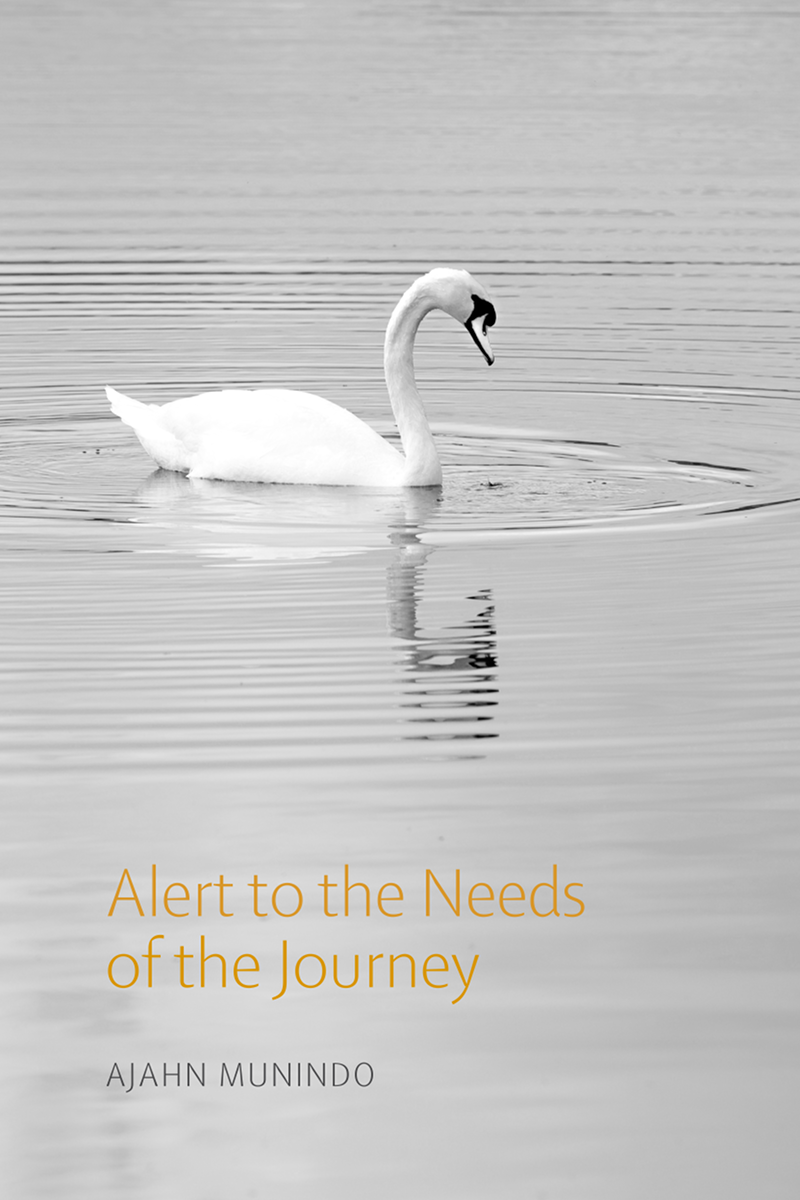
\includegraphics[height=\paperheight]{./desktop-cover.png}}
\fi

\cleartorecto
\thispagestyle{empty}
\vspace*{5em}

{\centering

\settowidth{\titleLength}{%
  {\Large\chapterTitleFont\scshape\MakeLowercase{\thetitle}}%
}

{\Large\chapterTitleFont\scshape\MakeLowercase{\thetitle}}\\[0.3\baselineskip]
\setlength{\xheight}{\heightof{X}}
\raisebox{0.5\xheight}{\color[gray]{0.4}\rule{\titleLength}{0.25pt}}\\[0.3\baselineskip]
{\itshape
\thesubtitle}

\vfill

\theauthor

\vspace*{5em}

}



\cleartoverso
\thispagestyle{empty}

{\copyrightsize
\raggedright
\setlength{\parindent}{0pt}%
\setlength{\parskip}{0.8\baselineskip}%

\thetitle\\
by \theauthor

This publication is made available\\
for free distribution\\
by Aruno Publications

Aruno Publications is administered by:\\
Harnham Buddhist Monastery Trust\\
Company No. 6688355,\\
Unincorporated Charity Reg. No. 1126476

Contact Aruno Publications at \href{https://ratanagiri.org.uk/}{www.ratanagiri.org.uk}\\
This book is available for free download at\\
\href{https://forestsangha.org/}{www.forestsangha.org}

ISBN \theISBN

Copyright \copyright\ Aruno Publications 2018

\vfill

{\footnotesize

This work is licensed under a Creative Commons\\
Attribution-NonCommercial-NoDerivatives 4.0 International~License.

Produced with the \LaTeX\ typesetting system, set in Gentium, Shaker,\\
Merriweather and Hattori Hanzo.

\theEditionInfo

}}


\cleartorecto
\thispagestyle{empty}

\mbox{}\vfill

\begin{verse}

{\itshape
Lorem ipsum dolor sit amet,\\
consectetuer adipiscing elit.
}


\end{verse}

\vfill\mbox{}


\cleartorecto
\tableofcontents*

\chapter{Foreword}

Nullam eu ante vel est convallis dignissim. Fusce suscipit, wisi nec facilisis
facilisis, est dui fermentum leo, quis tempor ligula erat quis odio. Nunc porta
vulputate tellus. Nunc rutrum turpis sed pede. Sed bibendum. Aliquam posuere.
Nunc aliquet, augue nec adipiscing interdum, lacus tellus malesuada massa, quis
varius mi purus non odio. Pellentesque condimentum, magna ut suscipit hendrerit,
ipsum augue ornare nulla, non luctus diam neque sit amet urna. Curabitur
vulputate vestibulum lorem. Fusce sagittis, libero non molestie mollis, magna
orci ultrices dolor, at vulputate neque nulla lacinia eros. Sed id ligula quis
est convallis tempor. Curabitur lacinia pulvinar nibh. Nam a sapien.

\bigskip

{\raggedleft
  Reviewer Person\\
  July 2017
\par}


\chapter{Preface}

Nullam eu ante vel est convallis dignissim. Fusce suscipit, wisi nec facilisis
facilisis, est dui fermentum leo, quis tempor ligula erat quis odio. Nunc porta
vulputate tellus. Nunc rutrum turpis sed pede. Sed bibendum. Aliquam posuere.
Nunc aliquet, augue nec adipiscing interdum, lacus tellus malesuada massa, quis
varius mi purus non odio. Pellentesque condimentum, magna ut suscipit hendrerit,
ipsum augue ornare nulla, non luctus diam neque sit amet urna. Curabitur
vulputate vestibulum lorem. Fusce sagittis, libero non molestie mollis, magna
orci ultrices dolor, at vulputate neque nulla lacinia eros. Sed id ligula quis
est convallis tempor. Curabitur lacinia pulvinar nibh. Nam a sapien.

\bigskip

{\raggedleft
  The Author\\
  July 2017
\par}



% Page 1 is the first page of the first chapter.
\mainmatter

\chapterNote{Chapter one subtitle}

\chapter{Chapter One Title}
\tocChapterNote{Chapter one subtitle}

Aliquam erat volutpat. Nunc eleifend leo vitae magna. In id erat non orci
commodo lobortis. Proin neque massa, cursus ut, gravida ut, lobortis eget,
lacus. Sed diam. Praesent fermentum tempor tellus. Nullam tempus. Mauris ac
felis vel velit tristique imperdiet. Donec at pede. Etiam vel neque nec dui
dignissim bibendum. Vivamus id enim. Phasellus neque orci, porta a, aliquet
quis, semper a, massa. Phasellus purus. Pellentesque tristique imperdiet tortor.
Nam euismod tellus id erat.


\chapterNote{Chapter two subtitle}

\chapter{Chapter Two Title}
\tocChapterNote{Chapter two subtitle}

Nullam eu ante vel est convallis dignissim. Fusce suscipit, wisi nec facilisis
facilisis, est dui fermentum leo, quis tempor ligula erat quis odio. Nunc porta
vulputate tellus. Nunc rutrum turpis sed pede. Sed bibendum. Aliquam posuere.
Nunc aliquet, augue nec adipiscing interdum, lacus tellus malesuada massa, quis
varius mi purus non odio. Pellentesque condimentum, magna ut suscipit hendrerit,
ipsum augue ornare nulla, non luctus diam neque sit amet urna. Curabitur
vulputate vestibulum lorem. Fusce sagittis, libero non molestie mollis, magna
orci ultrices dolor, at vulputate neque nulla lacinia eros. Sed id ligula quis
est convallis tempor. Curabitur lacinia pulvinar nibh. Nam a sapien.




\backmatter

\chapter{Glossary}

\begin{glossarydescription}

% === A ===

\item[anicca] (Pali) Impermanence: one of the \emph{three characteristics of
    existence} along with not-self (\emph{anattā}) and unsatisfactoriness
  (\emph{dukkha}).

% === B ===

\item[borapet] (Thai) Tinospora crispa. Heart-shaped moonseed or guduchi.
  An extremely bitter vine used as a prophylactic and treatment for malaria.

% === C ===

% === D ===

% === E ===

% === F ===

% === G ===

% === H ===

% === I ===

% === J ===

% === K ===

% === L ===

% === M ===

% === N ===

% === O ===

% === P ===

% === Q ===

% === R ===

% === S ===

% === T ===

% === U ===

% === V ===

% === W ===

\end{glossarydescription}



\cleartorecto
\thispagestyle{plain}

{\fontsize{9.5}{13.5}\selectfont%
\setlength{\parindent}{0pt}%
\raggedright\label{copyright-details}%
\setlength{\parskip}{7pt}%

{\centering

{\LARGE\ccbyncnd}

This work is licensed under a Creative Commons\\
Attribution-NonCommercial-NoDerivatives 4.0 International~License.\footnote{%
\href{https://creativecommons.org/licenses/by-nc-nd/4.0/}{https://creativecommons.org/licenses/by-nc-nd/4.0/}}

}

You are free to:

\begin{packeditemize}
\item Share — copy and redistribute the material in any medium or format
\end{packeditemize}

The licensor cannot revoke these freedoms as long as you follow the license terms.

Under the following terms:

\begin{packeditemize}
\item Attribution — You must give appropriate credit, provide a link to the license, and indicate if changes were made. You may do so in any reasonable manner, but not in any way that suggests the licensor endorses you or your use.
\item NonCommercial — You may not use the material for commercial purposes.
\item NoDerivatives — If you remix, transform, or build upon the material, you may not distribute the modified material.
\end{packeditemize}

No additional restrictions — You may not apply legal terms or technological measures that legally restrict others from doing anything the license permits.

Notices:

You do not have to comply with the license for elements of the material in the public domain or where your use is permitted by an applicable exception or limitation.

No warranties are given. The license may not give you all of the permissions necessary for your intended use. For example, other rights such as publicity, privacy, or moral rights may limit how you use the material.

Harnham Buddhist Monastery Trust operating as Aruno Publications asserts its moral right to be identified as the author of this book.

Harnham Buddhist Monastery Trust requests that you attribute ownership of the work to Aruno Publications on copying, distribution, display or performance of the work.

}

\emptyUntilModEight

\end{document}
